\documentclass[twoside]{book}

% Packages required by doxygen
\usepackage{fixltx2e}
\usepackage{calc}
\usepackage{doxygen}
\usepackage[export]{adjustbox} % also loads graphicx
\usepackage{graphicx}
\usepackage[utf8]{inputenc}
\usepackage{makeidx}
\usepackage{multicol}
\usepackage{multirow}
\PassOptionsToPackage{warn}{textcomp}
\usepackage{textcomp}
\usepackage[nointegrals]{wasysym}
\usepackage[table]{xcolor}

% Font selection
\usepackage[T1]{fontenc}
\usepackage[scaled=.90]{helvet}
\usepackage{courier}
\usepackage{amssymb}
\usepackage{sectsty}
\renewcommand{\familydefault}{\sfdefault}
\allsectionsfont{%
  \fontseries{bc}\selectfont%
  \color{darkgray}%
}
\renewcommand{\DoxyLabelFont}{%
  \fontseries{bc}\selectfont%
  \color{darkgray}%
}
\newcommand{\+}{\discretionary{\mbox{\scriptsize$\hookleftarrow$}}{}{}}

% Page & text layout
\usepackage{geometry}
\geometry{%
  a4paper,%
  top=2.5cm,%
  bottom=2.5cm,%
  left=2.5cm,%
  right=2.5cm%
}
\tolerance=750
\hfuzz=15pt
\hbadness=750
\setlength{\emergencystretch}{15pt}
\setlength{\parindent}{0cm}
\setlength{\parskip}{3ex plus 2ex minus 2ex}
\makeatletter
\renewcommand{\paragraph}{%
  \@startsection{paragraph}{4}{0ex}{-1.0ex}{1.0ex}{%
    \normalfont\normalsize\bfseries\SS@parafont%
  }%
}
\renewcommand{\subparagraph}{%
  \@startsection{subparagraph}{5}{0ex}{-1.0ex}{1.0ex}{%
    \normalfont\normalsize\bfseries\SS@subparafont%
  }%
}
\makeatother

% Headers & footers
\usepackage{fancyhdr}
\pagestyle{fancyplain}
\fancyhead[LE]{\fancyplain{}{\bfseries\thepage}}
\fancyhead[CE]{\fancyplain{}{}}
\fancyhead[RE]{\fancyplain{}{\bfseries\leftmark}}
\fancyhead[LO]{\fancyplain{}{\bfseries\rightmark}}
\fancyhead[CO]{\fancyplain{}{}}
\fancyhead[RO]{\fancyplain{}{\bfseries\thepage}}
\fancyfoot[LE]{\fancyplain{}{}}
\fancyfoot[CE]{\fancyplain{}{}}
\fancyfoot[RE]{\fancyplain{}{\bfseries\scriptsize Generated by Doxygen }}
\fancyfoot[LO]{\fancyplain{}{\bfseries\scriptsize Generated by Doxygen }}
\fancyfoot[CO]{\fancyplain{}{}}
\fancyfoot[RO]{\fancyplain{}{}}
\renewcommand{\footrulewidth}{0.4pt}
\renewcommand{\chaptermark}[1]{%
  \markboth{#1}{}%
}
\renewcommand{\sectionmark}[1]{%
  \markright{\thesection\ #1}%
}

% Indices & bibliography
\usepackage{natbib}
\usepackage[titles]{tocloft}
\setcounter{tocdepth}{3}
\setcounter{secnumdepth}{5}
\makeindex

% Hyperlinks (required, but should be loaded last)
\usepackage{ifpdf}
\ifpdf
  \usepackage[pdftex,pagebackref=true]{hyperref}
\else
  \usepackage[ps2pdf,pagebackref=true]{hyperref}
\fi
\hypersetup{%
  colorlinks=true,%
  linkcolor=blue,%
  citecolor=blue,%
  unicode%
}

% Custom commands
\newcommand{\clearemptydoublepage}{%
  \newpage{\pagestyle{empty}\cleardoublepage}%
}

\usepackage{caption}
\captionsetup{labelsep=space,justification=centering,font={bf},singlelinecheck=off,skip=4pt,position=top}

%===== C O N T E N T S =====

\begin{document}

% Titlepage & ToC
\hypersetup{pageanchor=false,
             bookmarksnumbered=true,
             pdfencoding=unicode
            }
\pagenumbering{roman}
\begin{titlepage}
\vspace*{7cm}
\begin{center}%
{\Large P\+E\+C\+A\+NS (Python Ediable Chemical Atmospheric Numerical Solver) }\\
\vspace*{1cm}
{\large Generated by Doxygen 1.8.11}\\
\end{center}
\end{titlepage}
\clearemptydoublepage
\tableofcontents
\clearemptydoublepage
\pagenumbering{arabic}
\hypersetup{pageanchor=true}

%--- Begin generated contents ---
\chapter{Preface}
\label{md_additional_1-pecans_front_matter}
\hypertarget{md_additional_1-pecans_front_matter}{}
\subsection*{P\+E\+C\+A\+NS\+: the Python Editable Chemical Atmospheric Numeric Solver}

The goal of the P\+E\+C\+A\+NS multi-\/box model is to provide a relatively straightforward but efficient and flexible idealized atmospheric chemistry modeling framework. It is not intended to supplant global or regional chemical transport models such as G\+E\+O\+S-\/\+Chem, W\+R\+F-\/\+Chem, or C\+M\+AQ, but instead to offer the capability to carry out one box to 3D multi-\/box modeling with idealized (rather than real world) transport.

Keeping the code base clean and easy to follow is a top priority for this model. This is why we have chosen to develop the code in Python/\+Cython rather than Fortran or C, and we will be aggressively documenting the behavior of the model. The code will also be written with the \char`\"{}code is written once, read many times\char`\"{} philosophy.

Most users should be able to use P\+E\+C\+A\+NS in their research without modifying the code at all, by modifying the mechanism and configuration files. However, this guide will be written with the expectation that at least some users will want to inspect the code, either to understand how it works, troubleshoot the behavior of the model, or to extend the behavior in some manner. Thus, the later chapters of this documentation will include information about the progammatic structure of the model, as well as the necessary information for end users.

\subsection*{Obtaining}

The P\+E\+C\+A\+NS model can be obtained from the Git\+Hub repository at

\href{https://github.com/firsttempora/PECANS}{\tt https\+://github.\+com/firsttempora/\+P\+E\+C\+A\+NS}

We recommend that you clone the repository, this will allow you to receive updates most easily. However, you may also download one of the \href{https://github.com/firsttempora/PECANS/releases}{\tt releases}.

\subsection*{Reporting problems or contacting us}

The best way to report a problem is via the \href{https://github.com/firsttempora/PECANS/issues}{\tt Issues} tab of the Git\+Hub repository. This ensures a record of the issue exists and will not be lost in an inbox somewhere.

If you have a question, it is best if you open an issue with the \char`\"{}question\char`\"{} tag. This way, there is a record of your question that may help another user and if it needs to be addressed through an update to the code, it will already be logged.

If you prefer to contact the author(s) directly, reach out to\+:

\href{mailto:first.tempora@gmail.com}{\tt first.\+tempora@gmail.\+com}

\subsection*{Contributing}

Contributions are welcome! If you would like to submit an improvement, please take the following steps\+:


\begin{DoxyEnumerate}
\item Read the style guide and follow the coding style laid out therein.
\item Consider if the improvement keeps the model {\itshape straightforward} and {\itshape flexible} (please contact us if you are uncertain if it does.)
\item \href{https://help.github.com/articles/fork-a-repo/}{\tt Fork} the Git\+Hub repository to your Git\+Hub account and clone the fork.
\item Make your modifications to the forked repository.
\item Submit a \href{https://help.github.com/articles/about-pull-requests/}{\tt pull request} 
\end{DoxyEnumerate}
\chapter{Getting started}
\label{md_additional_2-getting-started}
\hypertarget{md_additional_2-getting-started}{}
\subsection*{Quick start}

Assuming you want to use one of the built in mechanisms\+:


\begin{DoxyEnumerate}
\item (optional, but recommended) Set up a virtual environment (see below)
\item Clone/download the P\+E\+C\+A\+NS model
\item Install the required Python packages with {\ttfamily pip3 install -\/r requirements.\+txt}
\item Build a mechanism with the {\ttfamily build\+\_\+pecans.\+py} script (run it to select options interactively).
\item ({\itshape not yet implemented}) Execute the model with the {\ttfamily run\+\_\+pecans.\+py} script.
\end{DoxyEnumerate}

\subsection*{Detail start}

\subsubsection*{1) Set up a virtual environment (optional)}

Although this is optional, we do recommend that you set up P\+E\+C\+A\+NS in a Python 3 virtual environment if at all possible. This ensures that you can install the necessary packages without changing your system wide Python installation.

With a standard Python 3 installation, you create a virtual environment with the command {\ttfamily python3 -\/m venv My\+Virt\+Env}. This will create a folder {\ttfamily My\+Virt\+Env} in the current folder (you can change that name to whatever you wish).

Users with an Anaconda python installation may wish to use {\ttfamily conda create -\/-\/name My\+Virt\+Env} instead.

After creating the virtual environment, {\ttfamily cd} into that directory and type {\ttfamily source bin/activate} to activate that virtual environment. You will need to perform this step each time you wish to build or run the model, {\itshape if} you build it in a virtual environment.

The first time you activate the virtual environment, it\textquotesingle{}s a good idea to make sure {\ttfamily pip} (the Python package installer) is up to date by running the command {\ttfamily pip3 install -\/-\/upgrade pip}.

\subsubsection*{2) Clone or download the P\+E\+C\+A\+NS model}

I recommend you clone the model. That way you\textquotesingle{}ll be able to get any updates with a simple {\ttfamily git pull} command, and if you make any changes to the code, you\textquotesingle{}ll always be able to undo them. You will need \href{https://git-scm.com/downloads}{\tt git} installed on your computer. If you\textquotesingle{}d rather just download a compressed folder with the model, see the last paragraph.

To clone\+: open a terminal window and {\ttfamily cd} into your virtual environment folder (if you made one) or into a directory that you want the P\+E\+C\+A\+NS directory to exist in. Go to \href{https://github.com/firsttempora/PECANS}{\tt https\+://github.\+com/firsttempora/\+P\+E\+C\+A\+NS} and click the \char`\"{}\+Clone or download\char`\"{} button. Choose \char`\"{}\+H\+T\+T\+P\+S\char`\"{} and copy the link. Back in your terminal, type {\ttfamily git clone $<$link$>$}, pasting the link you just copied in place of {\ttfamily $<$link$>$} and press {\ttfamily enter}. Git will create a P\+E\+C\+A\+NS folder and download the model into it.

To download a compressed folder, go to the \href{https://github.com/firsttempora/PECANS/releases}{\tt releases} page of the Git\+Hub repo and download the most recent release. Decompress it with your favorite extractor.

\subsubsection*{3) Install the required Python packages}

P\+E\+C\+A\+NS has a number of packages it requires to run. All can be installed through the {\ttfamily pip3} utility. In the top P\+E\+C\+A\+NS folder, there is a {\ttfamily requirements.\+txt} document. With your virtual environment activated (if you made one), execute the command {\ttfamily pip3 install -\/r requirements.\+txt} from this folder. This tells {\ttfamily pip3} to install each of the dependencies listed in that file.

\subsubsection*{4) Build a mechanism}

The chemical mechanisms in P\+E\+C\+A\+NS are automatically coded into Cython from a mechanism file. This helps speed up computation by allowing the bulk of the program to be compiled and optimized. The process is automated by the {\ttfamily build\+\_\+pecans.\+py} script in the second P\+E\+C\+A\+NS folder under the main one. With your virtual environment activated (if you made one), execute this script with {\ttfamily ./build\+\_\+pecans.py} from the folder that it resides in. This will present you with a list of available mechanisms. Simply choose one and it will be build. You can also specify a mechanism on the command line, e.\+q. {\ttfamily ./build\+\_\+peacns.py nox} will build the \char`\"{}nox\char`\"{} mechanism. 
\chapter{Format for mechanism input files}
\label{md_additional_3-chemical_mech_format}
\hypertarget{md_additional_3-chemical_mech_format}{}
\subsection*{The basics}

Specifying a chemical mechanism requires at least two files\+:


\begin{DoxyItemize}
\item a {\ttfamily .spc} file that lists the species used in the reaction. (This helps catch typos in the next file.)
\item a {\ttfamily .eqn} file that lists the chemical reactions that occur and their rate constants.
\end{DoxyItemize}

By requiring the species file, the mechanism generator can verify that all the species used in the reactions are expected. If there is a typo, say \char`\"{}\+I\+S\+P\+O\char`\"{} instead of \char`\"{}\+I\+S\+O\+P\char`\"{} for isoprene, the parser can alert you to this, because \char`\"{}\+I\+S\+P\+O\char`\"{} is not a defined species.

There is one additional file that can be provided for each mechanism, which is a {\ttfamily .rate} file, which provides custom kinetic rate constants for that mechanism (more information below).

When you execute {\ttfamily build\+\_\+pecans.\+py}, it finds the corresponding {\ttfamily .spc}, {\ttfamily .eqn}, and {\ttfamily .rate} (if present) files in the pecans/\+Mechanisms folder. It passes these files to {\ttfamily mechgen.\+py} in the pecans/ folder. That in turn reads those files and generates {\ttfamily chemderiv.\+pyx}, a Cython source file. {\ttfamily build\+\_\+pecans.\+py} then runs the {\ttfamily setup.\+py} script in the same directory as itself to convert {\ttfamily chemderiv.\+pyx} into a {\ttfamily .c} source file and compile that into a binary executable. All the {\ttfamily chemderiv.$\ast$} files will be placed in the pecans/ folder.

\subsection*{P\+E\+C\+A\+NS format}

The native P\+E\+C\+A\+NS format for the mechanism files is designed to be extremely simple. It is very much modeled on the Kinetic Pre-\/processor (K\+PP) format used in W\+R\+F-\/\+Chem, but distilled down to its essence.

\subsubsection*{Species (.spc) file}

List each species used in the mechanism, one per line. Capitalization matters.

\subsubsection*{Reaction (.eqn) file}

List each reaction, one per line, e.\+g.\+: \begin{DoxyVerb}NO + O3 = NO2 : ARR2( 1.40e-12, 1310.0, TEMP )
\end{DoxyVerb}


The reaction itself is defined before the {\ttfamily \+:}. Reactants and products must be separated by {\itshape either} an {\ttfamily =} or {\ttfamily -\/$>$}, i.\+e. \begin{DoxyVerb}NO + O3 = NO2
\end{DoxyVerb}


is the same as \begin{DoxyVerb}NO + O3 -> NO2
\end{DoxyVerb}


Each reactant and product must be separated by a {\ttfamily +}. A coefficient of 1 may be omitted, as in the previous examples, while non-\/unity coefficients must come before the species name to which they apply, e.\+g. \begin{DoxyVerb}1.0 NO + 1.0 O3 = 1.0 NO2
\end{DoxyVerb}


The space between the coefficient and the name is optional. The coefficient must be written so that Python\textquotesingle{}s {\ttfamily float()} function can understand it; {\ttfamily 1}, {\ttfamily 1.\+0}, {\ttfamily 1e0}, {\ttfamily 1.\+0e0}, {\ttfamily -\/1}, etc. are all valid.

The rate constant for the reaction is given after the {\ttfamily \+:}. It can be one of three forms\+:


\begin{DoxyEnumerate}
\item A number that {\ttfamily float()} can intepret (see above for the coefficients)
\item A call to a function defined in one of the rates files (next section)
\item A string starting with {\ttfamily j} that indicates a photolysis rate ({\itshape not implemented})
\end{DoxyEnumerate}

In calls to a defined function, the variables {\ttfamily T\+E\+MP} and {\ttfamily C\+A\+IR} represent temperature in Kelvin and number density of air in molecules per cubic centimeter, respectively. E.\+g., \begin{DoxyVerb}ARR2( 1.40e-12, 1310.0, TEMP )
\end{DoxyVerb}


will call the {\ttfamily A\+R\+R2} function with temperature in Kelvin as the third argument.

\subsubsection*{Rates (.rate) file}

Reaction rates are, unfortunately, one place where it was necessary to require the user to accept a larger amount of complexity in order to provide sufficient flexibility in defining rate constants. Rate constant expressions can be defined as Cython {\ttfamily cdef} functions in two places\+:


\begin{DoxyEnumerate}
\item One of the {\ttfamily .rate} files in pecans/\+Rates. This is intended for standard rate constants distributed with the model.
\item A {\ttfamily .rate} file with the same name as the mechanism being compiled, stored in the pecans/\+Mechanisms folder. This is intended for user added reactions, although users are welcome to add custom files in the Rates folder for rate constant expressions which they wish to use across multiple reactions.
\end{DoxyEnumerate}

Rate expression must be written as valid Cython functions, specifically {\ttfamily cdef} functions (not {\ttfamily def} or {\ttfamily cpdef}, as {\ttfamily cdef} should be the fastest to call). These look similar to Python function definitions. An example is\+: \begin{DoxyVerb}cdef ko1d(double TEMP, double CAIR):
    cdef double kN
    cdef double k0

    kN = 0.78084 * CAIR * 1.8e-11 * exp(107 / TEMP)
    k0 = 0.20946 * CAIR * 3.2e-11 * exp(67 / TEMP)
    return kN + k0
\end{DoxyVerb}


The necessary parts are\+:
\begin{DoxyItemize}
\item The keyword {\ttfamily cdef} at the beginning
\item The name it will be called by ({\ttfamily ko1d} here)
\item The function arguments in parentheses ({\ttfamily T\+E\+MP} and {\ttfamily C\+A\+IR}), each preceeded by the type {\ttfamily double}.
\item A {\ttfamily \+:} after the closing parenthesis around the arguments
\item Any variables used within the function that are not inputs must be declared with the type declaration {\ttfamily cdef double}
\item Mathematical expression can be written using normal Python syntax (n.\+b. that raising to a power is done with {\ttfamily $\ast$$\ast$}, not {\ttfamily $^\wedge$}). The mathematical functions {\ttfamily exp}, {\ttfamily sqrt}, {\ttfamily log} (natural logarithm), and {\ttfamily log10} (log base 10) are available.
\item Return the final value of the rate constant with the {\ttfamily return} keyword.
\item For P\+E\+C\+A\+NS, temperature in Kelvin and number density of air in molec. / cm$^\wedge$3 must be the variables T\+E\+MP and C\+A\+IR, because the parser looks for those specifically to make sure their position matches in any calls in the {\ttfamily .eqn} file.
\end{DoxyItemize}

As many of these rate expression may be defined in a single {\ttfamily .rate} file as you wish. The parser will raise an exception if the same name is defined more than once across all {\ttfamily .rate} files read. 
\chapter{Namespace Index}
\section{Namespace List}
Here is a list of all documented namespaces with brief descriptions\+:\begin{DoxyCompactList}
\item\contentsline{section}{\hyperlink{namespacepecans}{pecans} }{\pageref{namespacepecans}}{}
\item\contentsline{section}{\hyperlink{namespacepecans_1_1mechgen}{pecans.\+mechgen} }{\pageref{namespacepecans_1_1mechgen}}{}
\end{DoxyCompactList}

\chapter{Hierarchical Index}
\section{Class Hierarchy}
This inheritance list is sorted roughly, but not completely, alphabetically\+:\begin{DoxyCompactList}
\item \contentsline{section}{pecans.\+mechgen.\+Derivative}{\pageref{classpecans_1_1mechgen_1_1Derivative}}{}
\item Exception\begin{DoxyCompactList}
\item \contentsline{section}{pecans.\+mechgen.\+Chem\+Error}{\pageref{classpecans_1_1mechgen_1_1ChemError}}{}
\begin{DoxyCompactList}
\item \contentsline{section}{pecans.\+mechgen.\+Rate\+Def\+Error}{\pageref{classpecans_1_1mechgen_1_1RateDefError}}{}
\item \contentsline{section}{pecans.\+mechgen.\+Reaction\+Def\+Error}{\pageref{classpecans_1_1mechgen_1_1ReactionDefError}}{}
\item \contentsline{section}{pecans.\+mechgen.\+Species\+Def\+Error}{\pageref{classpecans_1_1mechgen_1_1SpeciesDefError}}{}
\end{DoxyCompactList}
\end{DoxyCompactList}
\item \contentsline{section}{pecans.\+mechgen.\+Rate\+Expression}{\pageref{classpecans_1_1mechgen_1_1RateExpression}}{}
\item \contentsline{section}{pecans.\+mechgen.\+Reaction}{\pageref{classpecans_1_1mechgen_1_1Reaction}}{}
\item \contentsline{section}{pecans.\+mechgen.\+Reaction\+Specie}{\pageref{classpecans_1_1mechgen_1_1ReactionSpecie}}{}
\item \contentsline{section}{pecans.\+mechgen.\+Specie}{\pageref{classpecans_1_1mechgen_1_1Specie}}{}
\end{DoxyCompactList}

\chapter{Class Index}
\section{Class List}
Here are the classes, structs, unions and interfaces with brief descriptions\+:\begin{DoxyCompactList}
\item\contentsline{section}{\hyperlink{classpecans_1_1mechgen_1_1ChemError}{pecans.\+mechgen.\+Chem\+Error} }{\pageref{classpecans_1_1mechgen_1_1ChemError}}{}
\item\contentsline{section}{\hyperlink{classpecans_1_1mechgen_1_1Derivative}{pecans.\+mechgen.\+Derivative} }{\pageref{classpecans_1_1mechgen_1_1Derivative}}{}
\item\contentsline{section}{\hyperlink{classpecans_1_1mechgen_1_1RateDefError}{pecans.\+mechgen.\+Rate\+Def\+Error} }{\pageref{classpecans_1_1mechgen_1_1RateDefError}}{}
\item\contentsline{section}{\hyperlink{classpecans_1_1mechgen_1_1RateExpression}{pecans.\+mechgen.\+Rate\+Expression} }{\pageref{classpecans_1_1mechgen_1_1RateExpression}}{}
\item\contentsline{section}{\hyperlink{classpecans_1_1mechgen_1_1Reaction}{pecans.\+mechgen.\+Reaction} }{\pageref{classpecans_1_1mechgen_1_1Reaction}}{}
\item\contentsline{section}{\hyperlink{classpecans_1_1mechgen_1_1ReactionDefError}{pecans.\+mechgen.\+Reaction\+Def\+Error} }{\pageref{classpecans_1_1mechgen_1_1ReactionDefError}}{}
\item\contentsline{section}{\hyperlink{classpecans_1_1mechgen_1_1ReactionSpecie}{pecans.\+mechgen.\+Reaction\+Specie} }{\pageref{classpecans_1_1mechgen_1_1ReactionSpecie}}{}
\item\contentsline{section}{\hyperlink{classpecans_1_1mechgen_1_1Specie}{pecans.\+mechgen.\+Specie} }{\pageref{classpecans_1_1mechgen_1_1Specie}}{}
\item\contentsline{section}{\hyperlink{classpecans_1_1mechgen_1_1SpeciesDefError}{pecans.\+mechgen.\+Species\+Def\+Error} }{\pageref{classpecans_1_1mechgen_1_1SpeciesDefError}}{}
\end{DoxyCompactList}

\chapter{Namespace Documentation}
\hypertarget{namespacepecans}{}\section{pecans Namespace Reference}
\label{namespacepecans}\index{pecans@{pecans}}
\subsection*{Namespaces}
\begin{DoxyCompactItemize}
\item 
 \hyperlink{namespacepecans_1_1mechgen}{mechgen}
\end{DoxyCompactItemize}


\subsection{Detailed Description}
\begin{DoxyVerb}PECANS: Python Editable Chemical Atmospheric Numeric Solver
\end{DoxyVerb}
 
\hypertarget{namespacepecans_1_1mechgen}{}\section{pecans.\+mechgen Namespace Reference}
\label{namespacepecans_1_1mechgen}\index{pecans.\+mechgen@{pecans.\+mechgen}}
\subsection*{Classes}
\begin{DoxyCompactItemize}
\item 
class \hyperlink{classpecans_1_1mechgen_1_1ChemError}{Chem\+Error}
\item 
class \hyperlink{classpecans_1_1mechgen_1_1Derivative}{Derivative}
\item 
class \hyperlink{classpecans_1_1mechgen_1_1RateDefError}{Rate\+Def\+Error}
\item 
class \hyperlink{classpecans_1_1mechgen_1_1RateExpression}{Rate\+Expression}
\item 
class \hyperlink{classpecans_1_1mechgen_1_1Reaction}{Reaction}
\item 
class \hyperlink{classpecans_1_1mechgen_1_1ReactionDefError}{Reaction\+Def\+Error}
\item 
class \hyperlink{classpecans_1_1mechgen_1_1ReactionSpecie}{Reaction\+Specie}
\item 
class \hyperlink{classpecans_1_1mechgen_1_1Specie}{Specie}
\item 
class \hyperlink{classpecans_1_1mechgen_1_1SpeciesDefError}{Species\+Def\+Error}
\end{DoxyCompactItemize}
\subsection*{Functions}
\begin{DoxyCompactItemize}
\item 
def \hyperlink{namespacepecans_1_1mechgen_a998050ad09f27de979fff1102f144e9b}{generate\+\_\+pecans\+\_\+mechanism} (species\+\_\+file, reactions\+\_\+file, extra\+\_\+rate\+\_\+def\+\_\+file=None)
\item 
def \hyperlink{namespacepecans_1_1mechgen_a537f570f89214d1eb4de4120fab77c99}{generate\+\_\+chemderiv\+\_\+file} (reactions)
\item 
def {\bfseries generate\+\_\+mechanism} (mechanism\+\_\+style, species\+\_\+file, reactions\+\_\+file, additional\+\_\+rates\+\_\+file=None)\hypertarget{namespacepecans_1_1mechgen_a63228ddf741593d74c7c36c253ccdfa4}{}\label{namespacepecans_1_1mechgen_a63228ddf741593d74c7c36c253ccdfa4}

\end{DoxyCompactItemize}
\subsection*{Variables}
\begin{DoxyCompactItemize}
\item 
{\bfseries derivative\+\_\+file} = os.\+path.\+join(\+\_\+mydir, \textquotesingle{}chemderiv.\+pyx\textquotesingle{})\hypertarget{namespacepecans_1_1mechgen_ad3768d39ff17a98fe5557dd8c5cc5906}{}\label{namespacepecans_1_1mechgen_ad3768d39ff17a98fe5557dd8c5cc5906}

\item 
string {\bfseries pyx\+\_\+indent} = \textquotesingle{} \textquotesingle{}\hypertarget{namespacepecans_1_1mechgen_a107402f8c195fb2e8890ed47f2dae3ae}{}\label{namespacepecans_1_1mechgen_a107402f8c195fb2e8890ed47f2dae3ae}

\item 
string {\bfseries temperature\+\_\+variable} = \textquotesingle{}T\+E\+MP\textquotesingle{}\hypertarget{namespacepecans_1_1mechgen_a44fbe59fd0452f44bb22af2fc8b743f4}{}\label{namespacepecans_1_1mechgen_a44fbe59fd0452f44bb22af2fc8b743f4}

\item 
string {\bfseries ndens\+\_\+air\+\_\+variable} = \textquotesingle{}C\+A\+IR\textquotesingle{}\hypertarget{namespacepecans_1_1mechgen_a3532815164cb3268406c9dbba06c8a77}{}\label{namespacepecans_1_1mechgen_a3532815164cb3268406c9dbba06c8a77}

\item 
{\bfseries rate\+\_\+expr\+\_\+include\+\_\+dir} = os.\+path.\+join(\+\_\+mydir, \textquotesingle{}Rates\textquotesingle{})\hypertarget{namespacepecans_1_1mechgen_a6f056fe0002af4ffb0420ea33aea4922}{}\label{namespacepecans_1_1mechgen_a6f056fe0002af4ffb0420ea33aea4922}

\item 
list {\bfseries c\+\_\+math\+\_\+fxns} = \mbox{[}\textquotesingle{}exp\textquotesingle{}, \textquotesingle{}sqrt\textquotesingle{}, \textquotesingle{}log\textquotesingle{}, \textquotesingle{}log10\textquotesingle{}\mbox{]}\hypertarget{namespacepecans_1_1mechgen_a4b2dfbb7822ac276236b377b13d58a5c}{}\label{namespacepecans_1_1mechgen_a4b2dfbb7822ac276236b377b13d58a5c}

\item 
dictionary {\bfseries style\+\_\+parse\+\_\+fxn\+\_\+dict} = \{\textquotesingle{}pecans\textquotesingle{}\+:\hyperlink{namespacepecans_1_1mechgen_a998050ad09f27de979fff1102f144e9b}{generate\+\_\+pecans\+\_\+mechanism}\}\hypertarget{namespacepecans_1_1mechgen_ac68d24dbdb0124e04d8d7d268711289c}{}\label{namespacepecans_1_1mechgen_ac68d24dbdb0124e04d8d7d268711289c}

\end{DoxyCompactItemize}


\subsection{Detailed Description}
\begin{DoxyVerb}Generate mechanism solver file from a KPP-like mechanism file or one following PECANS style
\end{DoxyVerb}
 

\subsection{Function Documentation}
\index{pecans\+::mechgen@{pecans\+::mechgen}!generate\+\_\+chemderiv\+\_\+file@{generate\+\_\+chemderiv\+\_\+file}}
\index{generate\+\_\+chemderiv\+\_\+file@{generate\+\_\+chemderiv\+\_\+file}!pecans\+::mechgen@{pecans\+::mechgen}}
\subsubsection[{\texorpdfstring{generate\+\_\+chemderiv\+\_\+file(reactions)}{generate_chemderiv_file(reactions)}}]{\setlength{\rightskip}{0pt plus 5cm}def pecans.\+mechgen.\+generate\+\_\+chemderiv\+\_\+file (
\begin{DoxyParamCaption}
\item[{}]{reactions}
\end{DoxyParamCaption}
)}\hypertarget{namespacepecans_1_1mechgen_a537f570f89214d1eb4de4120fab77c99}{}\label{namespacepecans_1_1mechgen_a537f570f89214d1eb4de4120fab77c99}
\begin{DoxyVerb}Generates the chemical derivative .pyx file that contains all the derivative functions
 and rate constant functions plus the interface function that should be called from
 another Python program.
:param reactions: a list of instances of Reactions
:return: nothing
\end{DoxyVerb}
 \index{pecans\+::mechgen@{pecans\+::mechgen}!generate\+\_\+pecans\+\_\+mechanism@{generate\+\_\+pecans\+\_\+mechanism}}
\index{generate\+\_\+pecans\+\_\+mechanism@{generate\+\_\+pecans\+\_\+mechanism}!pecans\+::mechgen@{pecans\+::mechgen}}
\subsubsection[{\texorpdfstring{generate\+\_\+pecans\+\_\+mechanism(species\+\_\+file, reactions\+\_\+file, extra\+\_\+rate\+\_\+def\+\_\+file=\+None)}{generate_pecans_mechanism(species_file, reactions_file, extra_rate_def_file=None)}}]{\setlength{\rightskip}{0pt plus 5cm}def pecans.\+mechgen.\+generate\+\_\+pecans\+\_\+mechanism (
\begin{DoxyParamCaption}
\item[{}]{species\+\_\+file, }
\item[{}]{reactions\+\_\+file, }
\item[{}]{extra\+\_\+rate\+\_\+def\+\_\+file = {\ttfamily None}}
\end{DoxyParamCaption}
)}\hypertarget{namespacepecans_1_1mechgen_a998050ad09f27de979fff1102f144e9b}{}\label{namespacepecans_1_1mechgen_a998050ad09f27de979fff1102f144e9b}
\begin{DoxyVerb}Main function that generates a mechanism file for the PECANS style inputs. Any other
input file style must have an equivalent primary function that reads rate expression
files, reads the species file, and reads the reactions file.
:param species_file: the file defining all the species included in the mechanism
:param reactions_file: the file defining the reactions that comprise the mechanism
:param *extra_rate_def_file: any additional files beyond those in the "Rates" subdirectory
 that define rate constant expressions.
:return:
\end{DoxyVerb}
 
\chapter{Class Documentation}
\hypertarget{classpecans_1_1mechgen_1_1ChemError}{}\section{pecans.\+mechgen.\+Chem\+Error Class Reference}
\label{classpecans_1_1mechgen_1_1ChemError}\index{pecans.\+mechgen.\+Chem\+Error@{pecans.\+mechgen.\+Chem\+Error}}


Inheritance diagram for pecans.\+mechgen.\+Chem\+Error\+:\nopagebreak
\begin{figure}[H]
\begin{center}
\leavevmode
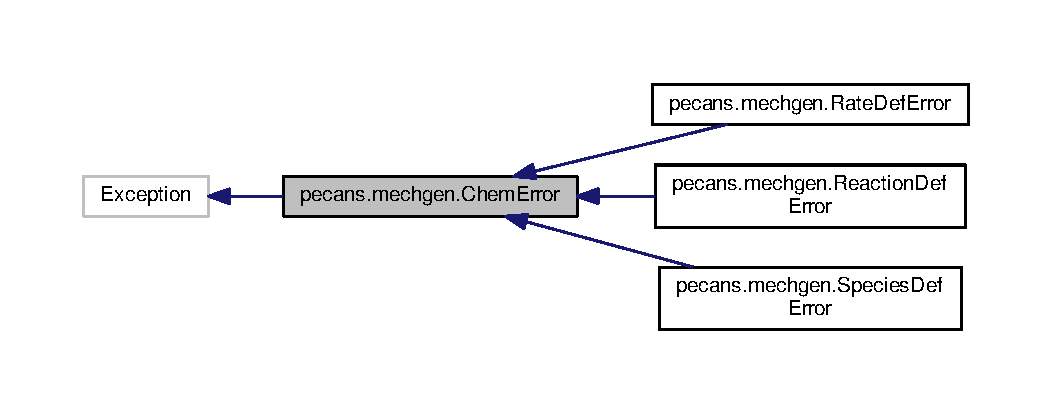
\includegraphics[width=350pt]{classpecans_1_1mechgen_1_1ChemError__inherit__graph}
\end{center}
\end{figure}


Collaboration diagram for pecans.\+mechgen.\+Chem\+Error\+:\nopagebreak
\begin{figure}[H]
\begin{center}
\leavevmode
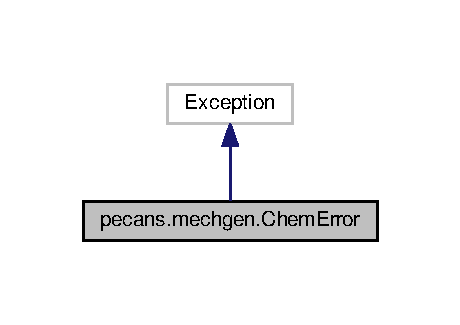
\includegraphics[width=221pt]{classpecans_1_1mechgen_1_1ChemError__coll__graph}
\end{center}
\end{figure}


The documentation for this class was generated from the following file\+:\begin{DoxyCompactItemize}
\item 
/home/josh/\+Documents/\+Python/\+Virt\+Envs/\+Chem\+Model/\+P\+E\+C\+A\+N\+S/pecans/mechgen.\+py\end{DoxyCompactItemize}

\hypertarget{classpecans_1_1mechgen_1_1Derivative}{}\section{pecans.\+mechgen.\+Derivative Class Reference}
\label{classpecans_1_1mechgen_1_1Derivative}\index{pecans.\+mechgen.\+Derivative@{pecans.\+mechgen.\+Derivative}}
\subsection*{Public Member Functions}
\begin{DoxyCompactItemize}
\item 
def \hyperlink{classpecans_1_1mechgen_1_1Derivative_a8e0a1ede8e4d02582dda60aa2738c4b7}{changed\+\_\+specie} (self)
\item 
def \hyperlink{classpecans_1_1mechgen_1_1Derivative_a262ef84f18366212ccfd65bf55e32e3f}{input\+\_\+species} (self)
\item 
def \hyperlink{classpecans_1_1mechgen_1_1Derivative_a1b27d7f388e6e23424d26131111d8eca}{reactions} (self)
\item 
def \hyperlink{classpecans_1_1mechgen_1_1Derivative_ad5d2c9c575a5f73dd1e8df55bde0b149}{coefficients} (self)
\item 
def \hyperlink{classpecans_1_1mechgen_1_1Derivative_a8e5fea94add3ea7b89af843e46a10f0d}{func\+\_\+signature} (self)
\item 
def \hyperlink{classpecans_1_1mechgen_1_1Derivative_aa36d38bcd95cd1788751b2c126ad54eb}{\+\_\+\+\_\+init\+\_\+\+\_\+} (self, specie)
\item 
def \hyperlink{classpecans_1_1mechgen_1_1Derivative_afd45c9243d14a3411bf0cd520eed89e8}{add\+\_\+rxn\+\_\+if\+\_\+relevant} (self, rxn)
\item 
def \hyperlink{classpecans_1_1mechgen_1_1Derivative_adde4d44f33a22c4785c1c1c989a06251}{finalize} (self)
\item 
def \hyperlink{classpecans_1_1mechgen_1_1Derivative_a68bc05227b54ff11d80ee283ee5895ba}{func\+\_\+def} (self)
\end{DoxyCompactItemize}


\subsection{Detailed Description}
\begin{DoxyVerb}Represents the derivative needed to calculate the change in a chemical specie
\end{DoxyVerb}
 

\subsection{Constructor \& Destructor Documentation}
\index{pecans\+::mechgen\+::\+Derivative@{pecans\+::mechgen\+::\+Derivative}!\+\_\+\+\_\+init\+\_\+\+\_\+@{\+\_\+\+\_\+init\+\_\+\+\_\+}}
\index{\+\_\+\+\_\+init\+\_\+\+\_\+@{\+\_\+\+\_\+init\+\_\+\+\_\+}!pecans\+::mechgen\+::\+Derivative@{pecans\+::mechgen\+::\+Derivative}}
\subsubsection[{\texorpdfstring{\+\_\+\+\_\+init\+\_\+\+\_\+(self, specie)}{__init__(self, specie)}}]{\setlength{\rightskip}{0pt plus 5cm}def pecans.\+mechgen.\+Derivative.\+\_\+\+\_\+init\+\_\+\+\_\+ (
\begin{DoxyParamCaption}
\item[{}]{self, }
\item[{}]{specie}
\end{DoxyParamCaption}
)}\hypertarget{classpecans_1_1mechgen_1_1Derivative_aa36d38bcd95cd1788751b2c126ad54eb}{}\label{classpecans_1_1mechgen_1_1Derivative_aa36d38bcd95cd1788751b2c126ad54eb}
\begin{DoxyVerb}Initialize an instance of Derivative that can be used to represent the change of a chemical
specie in a single timestep.
:param specie: The specie that the derivative is for; an instance of Specie
:return: an instance of Derivative
\end{DoxyVerb}
 

\subsection{Member Function Documentation}
\index{pecans\+::mechgen\+::\+Derivative@{pecans\+::mechgen\+::\+Derivative}!add\+\_\+rxn\+\_\+if\+\_\+relevant@{add\+\_\+rxn\+\_\+if\+\_\+relevant}}
\index{add\+\_\+rxn\+\_\+if\+\_\+relevant@{add\+\_\+rxn\+\_\+if\+\_\+relevant}!pecans\+::mechgen\+::\+Derivative@{pecans\+::mechgen\+::\+Derivative}}
\subsubsection[{\texorpdfstring{add\+\_\+rxn\+\_\+if\+\_\+relevant(self, rxn)}{add_rxn_if_relevant(self, rxn)}}]{\setlength{\rightskip}{0pt plus 5cm}def pecans.\+mechgen.\+Derivative.\+add\+\_\+rxn\+\_\+if\+\_\+relevant (
\begin{DoxyParamCaption}
\item[{}]{self, }
\item[{}]{rxn}
\end{DoxyParamCaption}
)}\hypertarget{classpecans_1_1mechgen_1_1Derivative_afd45c9243d14a3411bf0cd520eed89e8}{}\label{classpecans_1_1mechgen_1_1Derivative_afd45c9243d14a3411bf0cd520eed89e8}
\begin{DoxyVerb}Given a reaction, this will determine if the changed_specie appears on either side of the reaction
and if so, adds the reaction to the list of information that the derivative will need
:param rxn: an instance of Reaction
:return: a boolean, True if the reaction was relevant, False otherwise
\end{DoxyVerb}
 \index{pecans\+::mechgen\+::\+Derivative@{pecans\+::mechgen\+::\+Derivative}!changed\+\_\+specie@{changed\+\_\+specie}}
\index{changed\+\_\+specie@{changed\+\_\+specie}!pecans\+::mechgen\+::\+Derivative@{pecans\+::mechgen\+::\+Derivative}}
\subsubsection[{\texorpdfstring{changed\+\_\+specie(self)}{changed_specie(self)}}]{\setlength{\rightskip}{0pt plus 5cm}def pecans.\+mechgen.\+Derivative.\+changed\+\_\+specie (
\begin{DoxyParamCaption}
\item[{}]{self}
\end{DoxyParamCaption}
)}\hypertarget{classpecans_1_1mechgen_1_1Derivative_a8e0a1ede8e4d02582dda60aa2738c4b7}{}\label{classpecans_1_1mechgen_1_1Derivative_a8e0a1ede8e4d02582dda60aa2738c4b7}
\begin{DoxyVerb}The specie that the derivative is for
:return: an instance of Specie
\end{DoxyVerb}
 \index{pecans\+::mechgen\+::\+Derivative@{pecans\+::mechgen\+::\+Derivative}!coefficients@{coefficients}}
\index{coefficients@{coefficients}!pecans\+::mechgen\+::\+Derivative@{pecans\+::mechgen\+::\+Derivative}}
\subsubsection[{\texorpdfstring{coefficients(self)}{coefficients(self)}}]{\setlength{\rightskip}{0pt plus 5cm}def pecans.\+mechgen.\+Derivative.\+coefficients (
\begin{DoxyParamCaption}
\item[{}]{self}
\end{DoxyParamCaption}
)}\hypertarget{classpecans_1_1mechgen_1_1Derivative_ad5d2c9c575a5f73dd1e8df55bde0b149}{}\label{classpecans_1_1mechgen_1_1Derivative_ad5d2c9c575a5f73dd1e8df55bde0b149}
\begin{DoxyVerb}The coefficients for each reaction, tracking both how many molecules of the changed_specie
are produced or consumed and the sign (positive for produced, negative for consumed). This
is an overall coefficient, so if a specie appears on both sides, there will still be only
one coefficient for that reaction.
:return: a list of floats
\end{DoxyVerb}
 \index{pecans\+::mechgen\+::\+Derivative@{pecans\+::mechgen\+::\+Derivative}!finalize@{finalize}}
\index{finalize@{finalize}!pecans\+::mechgen\+::\+Derivative@{pecans\+::mechgen\+::\+Derivative}}
\subsubsection[{\texorpdfstring{finalize(self)}{finalize(self)}}]{\setlength{\rightskip}{0pt plus 5cm}def pecans.\+mechgen.\+Derivative.\+finalize (
\begin{DoxyParamCaption}
\item[{}]{self}
\end{DoxyParamCaption}
)}\hypertarget{classpecans_1_1mechgen_1_1Derivative_adde4d44f33a22c4785c1c1c989a06251}{}\label{classpecans_1_1mechgen_1_1Derivative_adde4d44f33a22c4785c1c1c989a06251}
\begin{DoxyVerb}To be called once all reactions are added. This, internally, converts the collection of input species
from a set to a tuple, to ensure that the order is consistent at all times.
:return: nothing
\end{DoxyVerb}
 \index{pecans\+::mechgen\+::\+Derivative@{pecans\+::mechgen\+::\+Derivative}!func\+\_\+def@{func\+\_\+def}}
\index{func\+\_\+def@{func\+\_\+def}!pecans\+::mechgen\+::\+Derivative@{pecans\+::mechgen\+::\+Derivative}}
\subsubsection[{\texorpdfstring{func\+\_\+def(self)}{func_def(self)}}]{\setlength{\rightskip}{0pt plus 5cm}def pecans.\+mechgen.\+Derivative.\+func\+\_\+def (
\begin{DoxyParamCaption}
\item[{}]{self}
\end{DoxyParamCaption}
)}\hypertarget{classpecans_1_1mechgen_1_1Derivative_a68bc05227b54ff11d80ee283ee5895ba}{}\label{classpecans_1_1mechgen_1_1Derivative_a68bc05227b54ff11d80ee283ee5895ba}
\begin{DoxyVerb}Creates the Cython function definition for the function that will calculate this derivative.
:return: A list of strings, each string is a line in the function definition
\end{DoxyVerb}
 \index{pecans\+::mechgen\+::\+Derivative@{pecans\+::mechgen\+::\+Derivative}!func\+\_\+signature@{func\+\_\+signature}}
\index{func\+\_\+signature@{func\+\_\+signature}!pecans\+::mechgen\+::\+Derivative@{pecans\+::mechgen\+::\+Derivative}}
\subsubsection[{\texorpdfstring{func\+\_\+signature(self)}{func_signature(self)}}]{\setlength{\rightskip}{0pt plus 5cm}def pecans.\+mechgen.\+Derivative.\+func\+\_\+signature (
\begin{DoxyParamCaption}
\item[{}]{self}
\end{DoxyParamCaption}
)}\hypertarget{classpecans_1_1mechgen_1_1Derivative_a8e5fea94add3ea7b89af843e46a10f0d}{}\label{classpecans_1_1mechgen_1_1Derivative_a8e5fea94add3ea7b89af843e46a10f0d}
\begin{DoxyVerb}The signature of the function that will be called to calculate the derivative. Includes the
function name, argument types, and argument names, i.e. dNO_dt(double conc_NO, double conc_O3)
Only defined after calling finalize() on this instance.
:return: a string that represents the function signature
\end{DoxyVerb}
 \index{pecans\+::mechgen\+::\+Derivative@{pecans\+::mechgen\+::\+Derivative}!input\+\_\+species@{input\+\_\+species}}
\index{input\+\_\+species@{input\+\_\+species}!pecans\+::mechgen\+::\+Derivative@{pecans\+::mechgen\+::\+Derivative}}
\subsubsection[{\texorpdfstring{input\+\_\+species(self)}{input_species(self)}}]{\setlength{\rightskip}{0pt plus 5cm}def pecans.\+mechgen.\+Derivative.\+input\+\_\+species (
\begin{DoxyParamCaption}
\item[{}]{self}
\end{DoxyParamCaption}
)}\hypertarget{classpecans_1_1mechgen_1_1Derivative_a262ef84f18366212ccfd65bf55e32e3f}{}\label{classpecans_1_1mechgen_1_1Derivative_a262ef84f18366212ccfd65bf55e32e3f}
\begin{DoxyVerb}The species whose concentrations are needed as inputs to calculate the derivative
:return: a set of instances of Specie
\end{DoxyVerb}
 \index{pecans\+::mechgen\+::\+Derivative@{pecans\+::mechgen\+::\+Derivative}!reactions@{reactions}}
\index{reactions@{reactions}!pecans\+::mechgen\+::\+Derivative@{pecans\+::mechgen\+::\+Derivative}}
\subsubsection[{\texorpdfstring{reactions(self)}{reactions(self)}}]{\setlength{\rightskip}{0pt plus 5cm}def pecans.\+mechgen.\+Derivative.\+reactions (
\begin{DoxyParamCaption}
\item[{}]{self}
\end{DoxyParamCaption}
)}\hypertarget{classpecans_1_1mechgen_1_1Derivative_a1b27d7f388e6e23424d26131111d8eca}{}\label{classpecans_1_1mechgen_1_1Derivative_a1b27d7f388e6e23424d26131111d8eca}
\begin{DoxyVerb}The reactions that involve the changed_specie
:return: a list of instances of Reaction
\end{DoxyVerb}
 

The documentation for this class was generated from the following file\+:\begin{DoxyCompactItemize}
\item 
/home/josh/\+Documents/\+Python/\+Virt\+Envs/\+Chem\+Model/\+P\+E\+C\+A\+N\+S/pecans/mechgen.\+py\end{DoxyCompactItemize}

\hypertarget{classpecans_1_1mechgen_1_1RateDefError}{}\section{pecans.\+mechgen.\+Rate\+Def\+Error Class Reference}
\label{classpecans_1_1mechgen_1_1RateDefError}\index{pecans.\+mechgen.\+Rate\+Def\+Error@{pecans.\+mechgen.\+Rate\+Def\+Error}}


Inheritance diagram for pecans.\+mechgen.\+Rate\+Def\+Error\+:\nopagebreak
\begin{figure}[H]
\begin{center}
\leavevmode
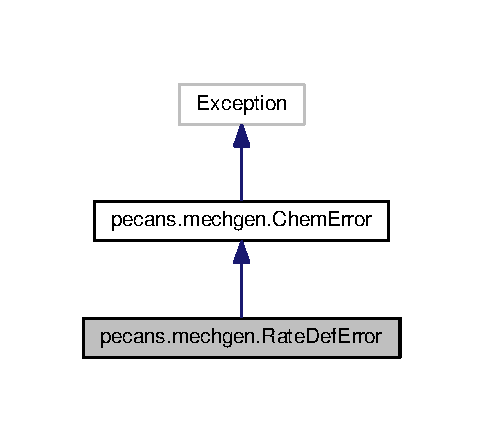
\includegraphics[width=232pt]{classpecans_1_1mechgen_1_1RateDefError__inherit__graph}
\end{center}
\end{figure}


Collaboration diagram for pecans.\+mechgen.\+Rate\+Def\+Error\+:\nopagebreak
\begin{figure}[H]
\begin{center}
\leavevmode
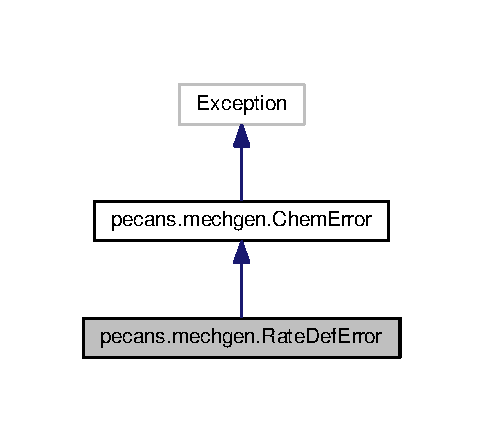
\includegraphics[width=232pt]{classpecans_1_1mechgen_1_1RateDefError__coll__graph}
\end{center}
\end{figure}


The documentation for this class was generated from the following file\+:\begin{DoxyCompactItemize}
\item 
/home/josh/\+Documents/\+Python/\+Virt\+Envs/\+Chem\+Model/\+P\+E\+C\+A\+N\+S/pecans/mechgen.\+py\end{DoxyCompactItemize}

\hypertarget{classpecans_1_1mechgen_1_1RateExpression}{}\section{pecans.\+mechgen.\+Rate\+Expression Class Reference}
\label{classpecans_1_1mechgen_1_1RateExpression}\index{pecans.\+mechgen.\+Rate\+Expression@{pecans.\+mechgen.\+Rate\+Expression}}
\subsection*{Public Member Functions}
\begin{DoxyCompactItemize}
\item 
def \hyperlink{classpecans_1_1mechgen_1_1RateExpression_aa70aebc347ad75a2d7a0ceeb652e6f6e}{\+\_\+\+\_\+init\+\_\+\+\_\+} (self, rate\+\_\+string, rate\+\_\+file, file\+\_\+line\+\_\+number)
\item 
def \hyperlink{classpecans_1_1mechgen_1_1RateExpression_a5f155e602ddebc7fd0a0e4b0a9f29cd9}{find\+\_\+rate\+\_\+by\+\_\+name} (cls, rate\+\_\+name)
\item 
def \hyperlink{classpecans_1_1mechgen_1_1RateExpression_af803879fa43b9fd746bfd9b66c4d2d1f}{mark\+\_\+rate\+\_\+as\+\_\+needed} (cls, rate\+\_\+call)
\end{DoxyCompactItemize}
\subsection*{Public Attributes}
\begin{DoxyCompactItemize}
\item 
{\bfseries used\+\_\+in\+\_\+mech}\hypertarget{classpecans_1_1mechgen_1_1RateExpression_ab04894c55dbe0031041e9ebe05dc8006}{}\label{classpecans_1_1mechgen_1_1RateExpression_ab04894c55dbe0031041e9ebe05dc8006}

\item 
{\bfseries declaring\+\_\+file}\hypertarget{classpecans_1_1mechgen_1_1RateExpression_a59cb46348e550bd9a06e059944c51c03}{}\label{classpecans_1_1mechgen_1_1RateExpression_a59cb46348e550bd9a06e059944c51c03}

\item 
{\bfseries file\+\_\+line}\hypertarget{classpecans_1_1mechgen_1_1RateExpression_a4bcc39375f52db34b759c1e88f6fb09e}{}\label{classpecans_1_1mechgen_1_1RateExpression_a4bcc39375f52db34b759c1e88f6fb09e}

\item 
{\bfseries ndens\+\_\+air\+\_\+ind}\hypertarget{classpecans_1_1mechgen_1_1RateExpression_a9713cbbd3d721163756021e5f5265ce3}{}\label{classpecans_1_1mechgen_1_1RateExpression_a9713cbbd3d721163756021e5f5265ce3}

\item 
{\bfseries body}\hypertarget{classpecans_1_1mechgen_1_1RateExpression_a76025977020514b92885973477e94fd2}{}\label{classpecans_1_1mechgen_1_1RateExpression_a76025977020514b92885973477e94fd2}

\item 
{\bfseries rate\+\_\+name}\hypertarget{classpecans_1_1mechgen_1_1RateExpression_a0c87729fceb6f1c26de999ff99c82544}{}\label{classpecans_1_1mechgen_1_1RateExpression_a0c87729fceb6f1c26de999ff99c82544}

\end{DoxyCompactItemize}
\subsection*{Static Public Attributes}
\begin{DoxyCompactItemize}
\item 
list {\bfseries instances} = \mbox{[}$\,$\mbox{]}\hypertarget{classpecans_1_1mechgen_1_1RateExpression_aab61de56261423df2138b7f354ce831a}{}\label{classpecans_1_1mechgen_1_1RateExpression_aab61de56261423df2138b7f354ce831a}

\end{DoxyCompactItemize}


\subsection{Detailed Description}
\begin{DoxyVerb}Class that holds all the defined rate constant expression functions
\end{DoxyVerb}
 

\subsection{Constructor \& Destructor Documentation}
\index{pecans\+::mechgen\+::\+Rate\+Expression@{pecans\+::mechgen\+::\+Rate\+Expression}!\+\_\+\+\_\+init\+\_\+\+\_\+@{\+\_\+\+\_\+init\+\_\+\+\_\+}}
\index{\+\_\+\+\_\+init\+\_\+\+\_\+@{\+\_\+\+\_\+init\+\_\+\+\_\+}!pecans\+::mechgen\+::\+Rate\+Expression@{pecans\+::mechgen\+::\+Rate\+Expression}}
\subsubsection[{\texorpdfstring{\+\_\+\+\_\+init\+\_\+\+\_\+(self, rate\+\_\+string, rate\+\_\+file, file\+\_\+line\+\_\+number)}{__init__(self, rate_string, rate_file, file_line_number)}}]{\setlength{\rightskip}{0pt plus 5cm}def pecans.\+mechgen.\+Rate\+Expression.\+\_\+\+\_\+init\+\_\+\+\_\+ (
\begin{DoxyParamCaption}
\item[{}]{self, }
\item[{}]{rate\+\_\+string, }
\item[{}]{rate\+\_\+file, }
\item[{}]{file\+\_\+line\+\_\+number}
\end{DoxyParamCaption}
)}\hypertarget{classpecans_1_1mechgen_1_1RateExpression_aa70aebc347ad75a2d7a0ceeb652e6f6e}{}\label{classpecans_1_1mechgen_1_1RateExpression_aa70aebc347ad75a2d7a0ceeb652e6f6e}
\begin{DoxyVerb}Create a new instance of RateExpression that holds information about a rate expression function.
That instance is stored in the class variable instances (RateExpression.instances), so there is
no need to store the returned instance.
:param rate_string: the string containing the entire function definition for the rate expression.
:param rate_file: the file that the definition was read from. Used to print more helpful error messages.
:param file_line_number: the line number in the file where the definition began. Again, for helpful error
messages.
:return: instance of RateExpression, which is also stored in RateExpression.instances.
\end{DoxyVerb}
 

\subsection{Member Function Documentation}
\index{pecans\+::mechgen\+::\+Rate\+Expression@{pecans\+::mechgen\+::\+Rate\+Expression}!find\+\_\+rate\+\_\+by\+\_\+name@{find\+\_\+rate\+\_\+by\+\_\+name}}
\index{find\+\_\+rate\+\_\+by\+\_\+name@{find\+\_\+rate\+\_\+by\+\_\+name}!pecans\+::mechgen\+::\+Rate\+Expression@{pecans\+::mechgen\+::\+Rate\+Expression}}
\subsubsection[{\texorpdfstring{find\+\_\+rate\+\_\+by\+\_\+name(cls, rate\+\_\+name)}{find_rate_by_name(cls, rate_name)}}]{\setlength{\rightskip}{0pt plus 5cm}def pecans.\+mechgen.\+Rate\+Expression.\+find\+\_\+rate\+\_\+by\+\_\+name (
\begin{DoxyParamCaption}
\item[{}]{cls, }
\item[{}]{rate\+\_\+name}
\end{DoxyParamCaption}
)}\hypertarget{classpecans_1_1mechgen_1_1RateExpression_a5f155e602ddebc7fd0a0e4b0a9f29cd9}{}\label{classpecans_1_1mechgen_1_1RateExpression_a5f155e602ddebc7fd0a0e4b0a9f29cd9}
\begin{DoxyVerb}Given a rate expression name, finds the instance that corresponds to it.
:param rate_name: The name of the rate expression, as a string
:return: the instance of RateExpression with that name. Raises a KeyError if one is not found.
\end{DoxyVerb}
 \index{pecans\+::mechgen\+::\+Rate\+Expression@{pecans\+::mechgen\+::\+Rate\+Expression}!mark\+\_\+rate\+\_\+as\+\_\+needed@{mark\+\_\+rate\+\_\+as\+\_\+needed}}
\index{mark\+\_\+rate\+\_\+as\+\_\+needed@{mark\+\_\+rate\+\_\+as\+\_\+needed}!pecans\+::mechgen\+::\+Rate\+Expression@{pecans\+::mechgen\+::\+Rate\+Expression}}
\subsubsection[{\texorpdfstring{mark\+\_\+rate\+\_\+as\+\_\+needed(cls, rate\+\_\+call)}{mark_rate_as_needed(cls, rate_call)}}]{\setlength{\rightskip}{0pt plus 5cm}def pecans.\+mechgen.\+Rate\+Expression.\+mark\+\_\+rate\+\_\+as\+\_\+needed (
\begin{DoxyParamCaption}
\item[{}]{cls, }
\item[{}]{rate\+\_\+call}
\end{DoxyParamCaption}
)}\hypertarget{classpecans_1_1mechgen_1_1RateExpression_af803879fa43b9fd746bfd9b66c4d2d1f}{}\label{classpecans_1_1mechgen_1_1RateExpression_af803879fa43b9fd746bfd9b66c4d2d1f}
\begin{DoxyVerb}Marks that the specified rate expression is used in the current mechanism, which causes it to be
inlined in the chemderiv.pyx file.
:param rate_call: the call to the rate expression, e.g. ARR2( 1.2e-12, 1310.0, TEMP )
:return: none
\end{DoxyVerb}
 

The documentation for this class was generated from the following file\+:\begin{DoxyCompactItemize}
\item 
/home/josh/\+Documents/\+Python/\+Virt\+Envs/\+Chem\+Model/\+P\+E\+C\+A\+N\+S/pecans/mechgen.\+py\end{DoxyCompactItemize}

\hypertarget{classpecans_1_1mechgen_1_1Reaction}{}\section{pecans.\+mechgen.\+Reaction Class Reference}
\label{classpecans_1_1mechgen_1_1Reaction}\index{pecans.\+mechgen.\+Reaction@{pecans.\+mechgen.\+Reaction}}
\subsection*{Public Member Functions}
\begin{DoxyCompactItemize}
\item 
def \hyperlink{classpecans_1_1mechgen_1_1Reaction_af015fb33f81a10a78d7e6ded5cf87be3}{id} (self)
\item 
def \hyperlink{classpecans_1_1mechgen_1_1Reaction_ac34f1f9597da3db1006890ca85e6d0a1}{reactants} (self)
\item 
def \hyperlink{classpecans_1_1mechgen_1_1Reaction_a8ee6cd94ee1de2c976232a5fa48d6c49}{reactant\+\_\+species} (self)
\item 
def \hyperlink{classpecans_1_1mechgen_1_1Reaction_a9890da73e627898c56c2fe1a09390e80}{products} (self)
\item 
def \hyperlink{classpecans_1_1mechgen_1_1Reaction_a1f6e4a9ad710e9a3636477a5d27a81c4}{product\+\_\+species} (self)
\item 
def \hyperlink{classpecans_1_1mechgen_1_1Reaction_ad25ecc71077556da29052f6afec9545f}{rate\+\_\+str} (self)
\item 
def \hyperlink{classpecans_1_1mechgen_1_1Reaction_adf16a0cf2950aab7ea62aefebcd4789f}{\+\_\+\+\_\+init\+\_\+\+\_\+} (self, \hyperlink{classpecans_1_1mechgen_1_1Reaction_ac34f1f9597da3db1006890ca85e6d0a1}{reactants}, \hyperlink{classpecans_1_1mechgen_1_1Reaction_a9890da73e627898c56c2fe1a09390e80}{products}, rate\+\_\+fxn)
\item 
def \hyperlink{classpecans_1_1mechgen_1_1Reaction_a9acdeaab1e5420929c7500e11c78b41d}{get\+\_\+reactant\+\_\+specie} (self, specie)
\item 
def \hyperlink{classpecans_1_1mechgen_1_1Reaction_a92487621cd9e2227ee81b4061caf502e}{get\+\_\+product\+\_\+specie} (self, specie)
\item 
def \hyperlink{classpecans_1_1mechgen_1_1Reaction_ae1abd8da5f183602e6ec3602bc7f2f22}{reset} (cls)
\item 
def {\bfseries \+\_\+\+\_\+str\+\_\+\+\_\+} (self)\hypertarget{classpecans_1_1mechgen_1_1Reaction_a074ffdf5307e850241772dbfa2c3d17a}{}\label{classpecans_1_1mechgen_1_1Reaction_a074ffdf5307e850241772dbfa2c3d17a}

\item 
def {\bfseries \+\_\+\+\_\+repr\+\_\+\+\_\+} (self)\hypertarget{classpecans_1_1mechgen_1_1Reaction_aa51f5848ba5bc1689c603dbc1a68192d}{}\label{classpecans_1_1mechgen_1_1Reaction_aa51f5848ba5bc1689c603dbc1a68192d}

\end{DoxyCompactItemize}
\subsection*{Public Attributes}
\begin{DoxyCompactItemize}
\item 
{\bfseries next\+\_\+id}\hypertarget{classpecans_1_1mechgen_1_1Reaction_a8d26627bd95499217692f691c2ec3d42}{}\label{classpecans_1_1mechgen_1_1Reaction_a8d26627bd95499217692f691c2ec3d42}

\end{DoxyCompactItemize}
\subsection*{Static Public Attributes}
\begin{DoxyCompactItemize}
\item 
int {\bfseries next\+\_\+id} = 0\hypertarget{classpecans_1_1mechgen_1_1Reaction_a86b4bbe81c34b5a34ab1c8ab660d8bfa}{}\label{classpecans_1_1mechgen_1_1Reaction_a86b4bbe81c34b5a34ab1c8ab660d8bfa}

\end{DoxyCompactItemize}


\subsection{Detailed Description}
\begin{DoxyVerb}Class representing chemical reactions in a mechanism
\end{DoxyVerb}
 

\subsection{Constructor \& Destructor Documentation}
\index{pecans\+::mechgen\+::\+Reaction@{pecans\+::mechgen\+::\+Reaction}!\+\_\+\+\_\+init\+\_\+\+\_\+@{\+\_\+\+\_\+init\+\_\+\+\_\+}}
\index{\+\_\+\+\_\+init\+\_\+\+\_\+@{\+\_\+\+\_\+init\+\_\+\+\_\+}!pecans\+::mechgen\+::\+Reaction@{pecans\+::mechgen\+::\+Reaction}}
\subsubsection[{\texorpdfstring{\+\_\+\+\_\+init\+\_\+\+\_\+(self, reactants, products, rate\+\_\+fxn)}{__init__(self, reactants, products, rate_fxn)}}]{\setlength{\rightskip}{0pt plus 5cm}def pecans.\+mechgen.\+Reaction.\+\_\+\+\_\+init\+\_\+\+\_\+ (
\begin{DoxyParamCaption}
\item[{}]{self, }
\item[{}]{reactants, }
\item[{}]{products, }
\item[{}]{rate\+\_\+fxn}
\end{DoxyParamCaption}
)}\hypertarget{classpecans_1_1mechgen_1_1Reaction_adf16a0cf2950aab7ea62aefebcd4789f}{}\label{classpecans_1_1mechgen_1_1Reaction_adf16a0cf2950aab7ea62aefebcd4789f}
\begin{DoxyVerb}Create an instance of Reaction that contains the reactants, products, and rate constant
:param reactants: a list, tuple, or set of instances of ReactionSpecie representing the reactants
:param products: a list, tuple, or set of instances of ReactionSpecie representing the products
:param rate_fxn: a representation of the rate constant, either as a function or value
:return: instance of Reaction
\end{DoxyVerb}
 

\subsection{Member Function Documentation}
\index{pecans\+::mechgen\+::\+Reaction@{pecans\+::mechgen\+::\+Reaction}!get\+\_\+product\+\_\+specie@{get\+\_\+product\+\_\+specie}}
\index{get\+\_\+product\+\_\+specie@{get\+\_\+product\+\_\+specie}!pecans\+::mechgen\+::\+Reaction@{pecans\+::mechgen\+::\+Reaction}}
\subsubsection[{\texorpdfstring{get\+\_\+product\+\_\+specie(self, specie)}{get_product_specie(self, specie)}}]{\setlength{\rightskip}{0pt plus 5cm}def pecans.\+mechgen.\+Reaction.\+get\+\_\+product\+\_\+specie (
\begin{DoxyParamCaption}
\item[{}]{self, }
\item[{}]{specie}
\end{DoxyParamCaption}
)}\hypertarget{classpecans_1_1mechgen_1_1Reaction_a92487621cd9e2227ee81b4061caf502e}{}\label{classpecans_1_1mechgen_1_1Reaction_a92487621cd9e2227ee81b4061caf502e}
\begin{DoxyVerb}Given an instance of Specie, returns the first corresponding product ReactionSpecie of that type of Specie
:param specie: an instance of Specie representing the chemical specie in question
:return: an instance of ReactionSpecie
\end{DoxyVerb}
 \index{pecans\+::mechgen\+::\+Reaction@{pecans\+::mechgen\+::\+Reaction}!get\+\_\+reactant\+\_\+specie@{get\+\_\+reactant\+\_\+specie}}
\index{get\+\_\+reactant\+\_\+specie@{get\+\_\+reactant\+\_\+specie}!pecans\+::mechgen\+::\+Reaction@{pecans\+::mechgen\+::\+Reaction}}
\subsubsection[{\texorpdfstring{get\+\_\+reactant\+\_\+specie(self, specie)}{get_reactant_specie(self, specie)}}]{\setlength{\rightskip}{0pt plus 5cm}def pecans.\+mechgen.\+Reaction.\+get\+\_\+reactant\+\_\+specie (
\begin{DoxyParamCaption}
\item[{}]{self, }
\item[{}]{specie}
\end{DoxyParamCaption}
)}\hypertarget{classpecans_1_1mechgen_1_1Reaction_a9acdeaab1e5420929c7500e11c78b41d}{}\label{classpecans_1_1mechgen_1_1Reaction_a9acdeaab1e5420929c7500e11c78b41d}
\begin{DoxyVerb}Given an instance of Specie, returns the first corresponding reactant ReactionSpecie of that type of Specie
:param specie: an instance of Specie representing the chemical specie in question
:return: an instance of ReactionSpecie
\end{DoxyVerb}
 \index{pecans\+::mechgen\+::\+Reaction@{pecans\+::mechgen\+::\+Reaction}!id@{id}}
\index{id@{id}!pecans\+::mechgen\+::\+Reaction@{pecans\+::mechgen\+::\+Reaction}}
\subsubsection[{\texorpdfstring{id(self)}{id(self)}}]{\setlength{\rightskip}{0pt plus 5cm}def pecans.\+mechgen.\+Reaction.\+id (
\begin{DoxyParamCaption}
\item[{}]{self}
\end{DoxyParamCaption}
)}\hypertarget{classpecans_1_1mechgen_1_1Reaction_af015fb33f81a10a78d7e6ded5cf87be3}{}\label{classpecans_1_1mechgen_1_1Reaction_af015fb33f81a10a78d7e6ded5cf87be3}
\begin{DoxyVerb}The unique numerical ID of the reaction
:return: the ID as an integer
\end{DoxyVerb}
 \index{pecans\+::mechgen\+::\+Reaction@{pecans\+::mechgen\+::\+Reaction}!product\+\_\+species@{product\+\_\+species}}
\index{product\+\_\+species@{product\+\_\+species}!pecans\+::mechgen\+::\+Reaction@{pecans\+::mechgen\+::\+Reaction}}
\subsubsection[{\texorpdfstring{product\+\_\+species(self)}{product_species(self)}}]{\setlength{\rightskip}{0pt plus 5cm}def pecans.\+mechgen.\+Reaction.\+product\+\_\+species (
\begin{DoxyParamCaption}
\item[{}]{self}
\end{DoxyParamCaption}
)}\hypertarget{classpecans_1_1mechgen_1_1Reaction_a1f6e4a9ad710e9a3636477a5d27a81c4}{}\label{classpecans_1_1mechgen_1_1Reaction_a1f6e4a9ad710e9a3636477a5d27a81c4}
\begin{DoxyVerb}Returns the unique species present as products
:return: a tuple of instances of Specie
\end{DoxyVerb}
 \index{pecans\+::mechgen\+::\+Reaction@{pecans\+::mechgen\+::\+Reaction}!products@{products}}
\index{products@{products}!pecans\+::mechgen\+::\+Reaction@{pecans\+::mechgen\+::\+Reaction}}
\subsubsection[{\texorpdfstring{products(self)}{products(self)}}]{\setlength{\rightskip}{0pt plus 5cm}def pecans.\+mechgen.\+Reaction.\+products (
\begin{DoxyParamCaption}
\item[{}]{self}
\end{DoxyParamCaption}
)}\hypertarget{classpecans_1_1mechgen_1_1Reaction_a9890da73e627898c56c2fe1a09390e80}{}\label{classpecans_1_1mechgen_1_1Reaction_a9890da73e627898c56c2fe1a09390e80}
\begin{DoxyVerb}Returns the products of the reaction
:return: a tuple of instances of ReactionSpecie
\end{DoxyVerb}
 \index{pecans\+::mechgen\+::\+Reaction@{pecans\+::mechgen\+::\+Reaction}!rate\+\_\+str@{rate\+\_\+str}}
\index{rate\+\_\+str@{rate\+\_\+str}!pecans\+::mechgen\+::\+Reaction@{pecans\+::mechgen\+::\+Reaction}}
\subsubsection[{\texorpdfstring{rate\+\_\+str(self)}{rate_str(self)}}]{\setlength{\rightskip}{0pt plus 5cm}def pecans.\+mechgen.\+Reaction.\+rate\+\_\+str (
\begin{DoxyParamCaption}
\item[{}]{self}
\end{DoxyParamCaption}
)}\hypertarget{classpecans_1_1mechgen_1_1Reaction_ad25ecc71077556da29052f6afec9545f}{}\label{classpecans_1_1mechgen_1_1Reaction_ad25ecc71077556da29052f6afec9545f}
\begin{DoxyVerb}Returns a representation of the rate constant as a string
NOTE: behavior may change
:return: a string, a number as a string or the name of the function given
\end{DoxyVerb}
 \index{pecans\+::mechgen\+::\+Reaction@{pecans\+::mechgen\+::\+Reaction}!reactant\+\_\+species@{reactant\+\_\+species}}
\index{reactant\+\_\+species@{reactant\+\_\+species}!pecans\+::mechgen\+::\+Reaction@{pecans\+::mechgen\+::\+Reaction}}
\subsubsection[{\texorpdfstring{reactant\+\_\+species(self)}{reactant_species(self)}}]{\setlength{\rightskip}{0pt plus 5cm}def pecans.\+mechgen.\+Reaction.\+reactant\+\_\+species (
\begin{DoxyParamCaption}
\item[{}]{self}
\end{DoxyParamCaption}
)}\hypertarget{classpecans_1_1mechgen_1_1Reaction_a8ee6cd94ee1de2c976232a5fa48d6c49}{}\label{classpecans_1_1mechgen_1_1Reaction_a8ee6cd94ee1de2c976232a5fa48d6c49}
\begin{DoxyVerb}Returns the unique species present as reactants
:return: a tuple of instances of Specie
\end{DoxyVerb}
 \index{pecans\+::mechgen\+::\+Reaction@{pecans\+::mechgen\+::\+Reaction}!reactants@{reactants}}
\index{reactants@{reactants}!pecans\+::mechgen\+::\+Reaction@{pecans\+::mechgen\+::\+Reaction}}
\subsubsection[{\texorpdfstring{reactants(self)}{reactants(self)}}]{\setlength{\rightskip}{0pt plus 5cm}def pecans.\+mechgen.\+Reaction.\+reactants (
\begin{DoxyParamCaption}
\item[{}]{self}
\end{DoxyParamCaption}
)}\hypertarget{classpecans_1_1mechgen_1_1Reaction_ac34f1f9597da3db1006890ca85e6d0a1}{}\label{classpecans_1_1mechgen_1_1Reaction_ac34f1f9597da3db1006890ca85e6d0a1}
\begin{DoxyVerb}Returns the reactants of the reaction
:return: a tuple of instances of ReactionSpecie
\end{DoxyVerb}
 \index{pecans\+::mechgen\+::\+Reaction@{pecans\+::mechgen\+::\+Reaction}!reset@{reset}}
\index{reset@{reset}!pecans\+::mechgen\+::\+Reaction@{pecans\+::mechgen\+::\+Reaction}}
\subsubsection[{\texorpdfstring{reset(cls)}{reset(cls)}}]{\setlength{\rightskip}{0pt plus 5cm}def pecans.\+mechgen.\+Reaction.\+reset (
\begin{DoxyParamCaption}
\item[{}]{cls}
\end{DoxyParamCaption}
)}\hypertarget{classpecans_1_1mechgen_1_1Reaction_ae1abd8da5f183602e6ec3602bc7f2f22}{}\label{classpecans_1_1mechgen_1_1Reaction_ae1abd8da5f183602e6ec3602bc7f2f22}
\begin{DoxyVerb}Restores the class variables to their initial state
:return: nothing
\end{DoxyVerb}
 

The documentation for this class was generated from the following file\+:\begin{DoxyCompactItemize}
\item 
/home/josh/\+Documents/\+Python/\+Virt\+Envs/\+Chem\+Model/\+P\+E\+C\+A\+N\+S/pecans/mechgen.\+py\end{DoxyCompactItemize}

\hypertarget{classpecans_1_1mechgen_1_1ReactionDefError}{}\section{pecans.\+mechgen.\+Reaction\+Def\+Error Class Reference}
\label{classpecans_1_1mechgen_1_1ReactionDefError}\index{pecans.\+mechgen.\+Reaction\+Def\+Error@{pecans.\+mechgen.\+Reaction\+Def\+Error}}


Inheritance diagram for pecans.\+mechgen.\+Reaction\+Def\+Error\+:\nopagebreak
\begin{figure}[H]
\begin{center}
\leavevmode
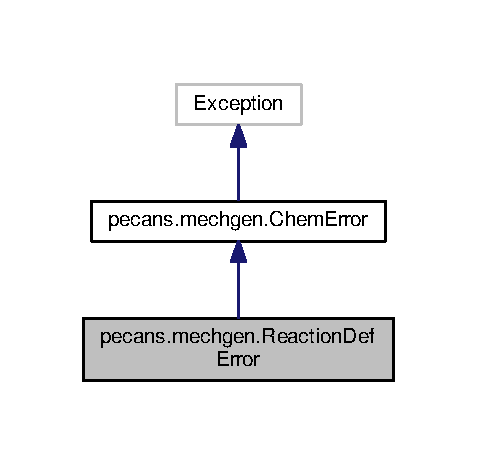
\includegraphics[width=229pt]{classpecans_1_1mechgen_1_1ReactionDefError__inherit__graph}
\end{center}
\end{figure}


Collaboration diagram for pecans.\+mechgen.\+Reaction\+Def\+Error\+:\nopagebreak
\begin{figure}[H]
\begin{center}
\leavevmode
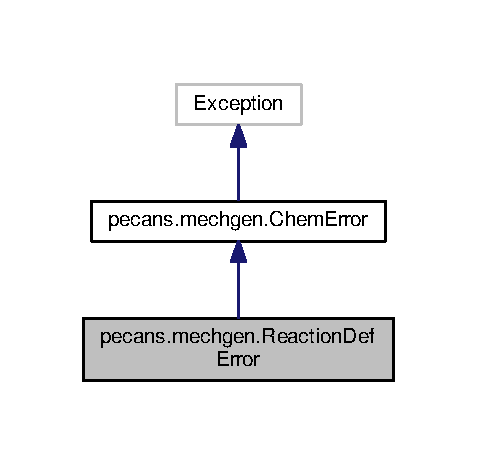
\includegraphics[width=229pt]{classpecans_1_1mechgen_1_1ReactionDefError__coll__graph}
\end{center}
\end{figure}


The documentation for this class was generated from the following file\+:\begin{DoxyCompactItemize}
\item 
/home/josh/\+Documents/\+Python/\+Virt\+Envs/\+Chem\+Model/\+P\+E\+C\+A\+N\+S/pecans/mechgen.\+py\end{DoxyCompactItemize}

\hypertarget{classpecans_1_1mechgen_1_1ReactionSpecie}{}\section{pecans.\+mechgen.\+Reaction\+Specie Class Reference}
\label{classpecans_1_1mechgen_1_1ReactionSpecie}\index{pecans.\+mechgen.\+Reaction\+Specie@{pecans.\+mechgen.\+Reaction\+Specie}}
\subsection*{Public Member Functions}
\begin{DoxyCompactItemize}
\item 
def {\bfseries specie} (self)\hypertarget{classpecans_1_1mechgen_1_1ReactionSpecie_ad46f5be87e846980da9dbed0bde770c0}{}\label{classpecans_1_1mechgen_1_1ReactionSpecie_ad46f5be87e846980da9dbed0bde770c0}

\item 
def {\bfseries name} (self)\hypertarget{classpecans_1_1mechgen_1_1ReactionSpecie_abfab8c1300934f4a9942b432f0183e2e}{}\label{classpecans_1_1mechgen_1_1ReactionSpecie_abfab8c1300934f4a9942b432f0183e2e}

\item 
def {\bfseries coefficient} (self)\hypertarget{classpecans_1_1mechgen_1_1ReactionSpecie_aa8abfaa343bd45881bcbe780386ad22f}{}\label{classpecans_1_1mechgen_1_1ReactionSpecie_aa8abfaa343bd45881bcbe780386ad22f}

\item 
def \hyperlink{classpecans_1_1mechgen_1_1ReactionSpecie_adcb988ca826c237283aa3974c5b09bd0}{\+\_\+\+\_\+init\+\_\+\+\_\+} (self, specie, coefficient=1.\+0)
\item 
def {\bfseries \+\_\+\+\_\+str\+\_\+\+\_\+} (self)\hypertarget{classpecans_1_1mechgen_1_1ReactionSpecie_a05b56bc3073c951a5c79b8bcda39653e}{}\label{classpecans_1_1mechgen_1_1ReactionSpecie_a05b56bc3073c951a5c79b8bcda39653e}

\item 
def {\bfseries \+\_\+\+\_\+repr\+\_\+\+\_\+} (self)\hypertarget{classpecans_1_1mechgen_1_1ReactionSpecie_a011550a386862e687b892f33b8f1890f}{}\label{classpecans_1_1mechgen_1_1ReactionSpecie_a011550a386862e687b892f33b8f1890f}

\end{DoxyCompactItemize}


\subsection{Detailed Description}
\begin{DoxyVerb}Wrapper class around Specie that matches it with a coefficient
\end{DoxyVerb}
 

\subsection{Constructor \& Destructor Documentation}
\index{pecans\+::mechgen\+::\+Reaction\+Specie@{pecans\+::mechgen\+::\+Reaction\+Specie}!\+\_\+\+\_\+init\+\_\+\+\_\+@{\+\_\+\+\_\+init\+\_\+\+\_\+}}
\index{\+\_\+\+\_\+init\+\_\+\+\_\+@{\+\_\+\+\_\+init\+\_\+\+\_\+}!pecans\+::mechgen\+::\+Reaction\+Specie@{pecans\+::mechgen\+::\+Reaction\+Specie}}
\subsubsection[{\texorpdfstring{\+\_\+\+\_\+init\+\_\+\+\_\+(self, specie, coefficient=1.\+0)}{__init__(self, specie, coefficient=1.0)}}]{\setlength{\rightskip}{0pt plus 5cm}def pecans.\+mechgen.\+Reaction\+Specie.\+\_\+\+\_\+init\+\_\+\+\_\+ (
\begin{DoxyParamCaption}
\item[{}]{self, }
\item[{}]{specie, }
\item[{}]{coefficient = {\ttfamily 1.0}}
\end{DoxyParamCaption}
)}\hypertarget{classpecans_1_1mechgen_1_1ReactionSpecie_adcb988ca826c237283aa3974c5b09bd0}{}\label{classpecans_1_1mechgen_1_1ReactionSpecie_adcb988ca826c237283aa3974c5b09bd0}
\begin{DoxyVerb}Create a new instance of ReactionSpecie that contains the given specie and
its coefficient in the reaction.
:param specie: An instance of Specie, representing the unique chemical specie in question
:param coefficient: The coefficient (as a float). Defaults to 1.0 if not given
:return: instance of ReactionSpecie
\end{DoxyVerb}
 

The documentation for this class was generated from the following file\+:\begin{DoxyCompactItemize}
\item 
/home/josh/\+Documents/\+Python/\+Virt\+Envs/\+Chem\+Model/\+P\+E\+C\+A\+N\+S/pecans/mechgen.\+py\end{DoxyCompactItemize}

\hypertarget{classpecans_1_1mechgen_1_1Specie}{}\section{pecans.\+mechgen.\+Specie Class Reference}
\label{classpecans_1_1mechgen_1_1Specie}\index{pecans.\+mechgen.\+Specie@{pecans.\+mechgen.\+Specie}}
\subsection*{Public Member Functions}
\begin{DoxyCompactItemize}
\item 
def \hyperlink{classpecans_1_1mechgen_1_1Specie_a41e559347b3423f3516301842385613c}{name} (self)
\item 
def \hyperlink{classpecans_1_1mechgen_1_1Specie_ad58b10b6479f367d6e33ef8744257445}{spec\+\_\+id} (self)
\item 
def \hyperlink{classpecans_1_1mechgen_1_1Specie_a4b9972921c40c021e7b56d5fc54324cc}{\+\_\+\+\_\+init\+\_\+\+\_\+} (self, \hyperlink{classpecans_1_1mechgen_1_1Specie_a41e559347b3423f3516301842385613c}{name})
\item 
def {\bfseries \+\_\+\+\_\+repr\+\_\+\+\_\+} (self)\hypertarget{classpecans_1_1mechgen_1_1Specie_a069a0d0e2f85bb2e7cf1f6471da4889e}{}\label{classpecans_1_1mechgen_1_1Specie_a069a0d0e2f85bb2e7cf1f6471da4889e}

\item 
def \hyperlink{classpecans_1_1mechgen_1_1Specie_a6901f1ddd421e3a9c8064b2800380415}{reset} (cls)
\item 
def \hyperlink{classpecans_1_1mechgen_1_1Specie_a34e33f51afc5238cbfcf73eeda600d99}{find\+\_\+by\+\_\+name} (cls, \hyperlink{classpecans_1_1mechgen_1_1Specie_a41e559347b3423f3516301842385613c}{name}, case\+\_\+sensitive=False)
\end{DoxyCompactItemize}
\subsection*{Public Attributes}
\begin{DoxyCompactItemize}
\item 
{\bfseries instances}\hypertarget{classpecans_1_1mechgen_1_1Specie_a2ec5debad50ea97e767e38ef840df970}{}\label{classpecans_1_1mechgen_1_1Specie_a2ec5debad50ea97e767e38ef840df970}

\item 
{\bfseries next\+\_\+id}\hypertarget{classpecans_1_1mechgen_1_1Specie_a3b362b20f1628091a44eae5325b4840a}{}\label{classpecans_1_1mechgen_1_1Specie_a3b362b20f1628091a44eae5325b4840a}

\end{DoxyCompactItemize}
\subsection*{Static Public Attributes}
\begin{DoxyCompactItemize}
\item 
list {\bfseries instances} = \mbox{[}$\,$\mbox{]}\hypertarget{classpecans_1_1mechgen_1_1Specie_ab94a7111e3f46171962598b5febaf96d}{}\label{classpecans_1_1mechgen_1_1Specie_ab94a7111e3f46171962598b5febaf96d}

\item 
int {\bfseries next\+\_\+id} = 0\hypertarget{classpecans_1_1mechgen_1_1Specie_a90532b3bc6c0be98e6cc2ea556f37309}{}\label{classpecans_1_1mechgen_1_1Specie_a90532b3bc6c0be98e6cc2ea556f37309}

\end{DoxyCompactItemize}


\subsection{Detailed Description}
\begin{DoxyVerb}Class which represents unique chemical species in the mechanism
\end{DoxyVerb}
 

\subsection{Constructor \& Destructor Documentation}
\index{pecans\+::mechgen\+::\+Specie@{pecans\+::mechgen\+::\+Specie}!\+\_\+\+\_\+init\+\_\+\+\_\+@{\+\_\+\+\_\+init\+\_\+\+\_\+}}
\index{\+\_\+\+\_\+init\+\_\+\+\_\+@{\+\_\+\+\_\+init\+\_\+\+\_\+}!pecans\+::mechgen\+::\+Specie@{pecans\+::mechgen\+::\+Specie}}
\subsubsection[{\texorpdfstring{\+\_\+\+\_\+init\+\_\+\+\_\+(self, name)}{__init__(self, name)}}]{\setlength{\rightskip}{0pt plus 5cm}def pecans.\+mechgen.\+Specie.\+\_\+\+\_\+init\+\_\+\+\_\+ (
\begin{DoxyParamCaption}
\item[{}]{self, }
\item[{}]{name}
\end{DoxyParamCaption}
)}\hypertarget{classpecans_1_1mechgen_1_1Specie_a4b9972921c40c021e7b56d5fc54324cc}{}\label{classpecans_1_1mechgen_1_1Specie_a4b9972921c40c021e7b56d5fc54324cc}
\begin{DoxyVerb}Create a new, unique species. Each instance is automatically registered with the
class variable "instances", and an error is thrown if the name matches one that
already exists.
:param name:
:return: instance of Specie
\end{DoxyVerb}
 

\subsection{Member Function Documentation}
\index{pecans\+::mechgen\+::\+Specie@{pecans\+::mechgen\+::\+Specie}!find\+\_\+by\+\_\+name@{find\+\_\+by\+\_\+name}}
\index{find\+\_\+by\+\_\+name@{find\+\_\+by\+\_\+name}!pecans\+::mechgen\+::\+Specie@{pecans\+::mechgen\+::\+Specie}}
\subsubsection[{\texorpdfstring{find\+\_\+by\+\_\+name(cls, name, case\+\_\+sensitive=\+False)}{find_by_name(cls, name, case_sensitive=False)}}]{\setlength{\rightskip}{0pt plus 5cm}def pecans.\+mechgen.\+Specie.\+find\+\_\+by\+\_\+name (
\begin{DoxyParamCaption}
\item[{}]{cls, }
\item[{}]{name, }
\item[{}]{case\+\_\+sensitive = {\ttfamily False}}
\end{DoxyParamCaption}
)}\hypertarget{classpecans_1_1mechgen_1_1Specie_a34e33f51afc5238cbfcf73eeda600d99}{}\label{classpecans_1_1mechgen_1_1Specie_a34e33f51afc5238cbfcf73eeda600d99}
\begin{DoxyVerb}Finds the species instance by its name
:param name: the name to search for
:param case_sensitive: if true, matches case, if false (default), does not
:return: an instance of Specie
\end{DoxyVerb}
 \index{pecans\+::mechgen\+::\+Specie@{pecans\+::mechgen\+::\+Specie}!name@{name}}
\index{name@{name}!pecans\+::mechgen\+::\+Specie@{pecans\+::mechgen\+::\+Specie}}
\subsubsection[{\texorpdfstring{name(self)}{name(self)}}]{\setlength{\rightskip}{0pt plus 5cm}def pecans.\+mechgen.\+Specie.\+name (
\begin{DoxyParamCaption}
\item[{}]{self}
\end{DoxyParamCaption}
)}\hypertarget{classpecans_1_1mechgen_1_1Specie_a41e559347b3423f3516301842385613c}{}\label{classpecans_1_1mechgen_1_1Specie_a41e559347b3423f3516301842385613c}
\begin{DoxyVerb}The name of the species
:return: the name as a string
\end{DoxyVerb}
 \index{pecans\+::mechgen\+::\+Specie@{pecans\+::mechgen\+::\+Specie}!reset@{reset}}
\index{reset@{reset}!pecans\+::mechgen\+::\+Specie@{pecans\+::mechgen\+::\+Specie}}
\subsubsection[{\texorpdfstring{reset(cls)}{reset(cls)}}]{\setlength{\rightskip}{0pt plus 5cm}def pecans.\+mechgen.\+Specie.\+reset (
\begin{DoxyParamCaption}
\item[{}]{cls}
\end{DoxyParamCaption}
)}\hypertarget{classpecans_1_1mechgen_1_1Specie_a6901f1ddd421e3a9c8064b2800380415}{}\label{classpecans_1_1mechgen_1_1Specie_a6901f1ddd421e3a9c8064b2800380415}
\begin{DoxyVerb}Clears the instances list and resets the ID counter
:return: nothing
\end{DoxyVerb}
 \index{pecans\+::mechgen\+::\+Specie@{pecans\+::mechgen\+::\+Specie}!spec\+\_\+id@{spec\+\_\+id}}
\index{spec\+\_\+id@{spec\+\_\+id}!pecans\+::mechgen\+::\+Specie@{pecans\+::mechgen\+::\+Specie}}
\subsubsection[{\texorpdfstring{spec\+\_\+id(self)}{spec_id(self)}}]{\setlength{\rightskip}{0pt plus 5cm}def pecans.\+mechgen.\+Specie.\+spec\+\_\+id (
\begin{DoxyParamCaption}
\item[{}]{self}
\end{DoxyParamCaption}
)}\hypertarget{classpecans_1_1mechgen_1_1Specie_ad58b10b6479f367d6e33ef8744257445}{}\label{classpecans_1_1mechgen_1_1Specie_ad58b10b6479f367d6e33ef8744257445}
\begin{DoxyVerb}The numerical ID of the species
:return: the ID as an integer
\end{DoxyVerb}
 

The documentation for this class was generated from the following file\+:\begin{DoxyCompactItemize}
\item 
/home/josh/\+Documents/\+Python/\+Virt\+Envs/\+Chem\+Model/\+P\+E\+C\+A\+N\+S/pecans/mechgen.\+py\end{DoxyCompactItemize}

\hypertarget{classpecans_1_1mechgen_1_1SpeciesDefError}{}\section{pecans.\+mechgen.\+Species\+Def\+Error Class Reference}
\label{classpecans_1_1mechgen_1_1SpeciesDefError}\index{pecans.\+mechgen.\+Species\+Def\+Error@{pecans.\+mechgen.\+Species\+Def\+Error}}


Inheritance diagram for pecans.\+mechgen.\+Species\+Def\+Error\+:\nopagebreak
\begin{figure}[H]
\begin{center}
\leavevmode
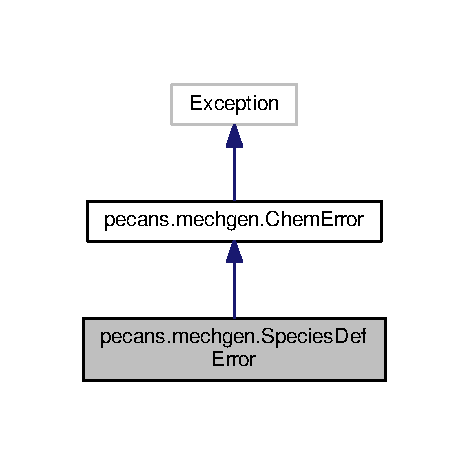
\includegraphics[width=225pt]{classpecans_1_1mechgen_1_1SpeciesDefError__inherit__graph}
\end{center}
\end{figure}


Collaboration diagram for pecans.\+mechgen.\+Species\+Def\+Error\+:\nopagebreak
\begin{figure}[H]
\begin{center}
\leavevmode
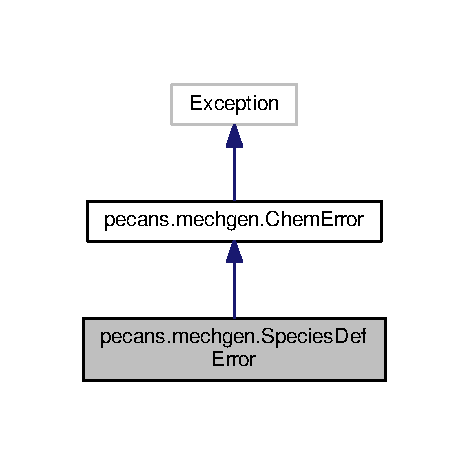
\includegraphics[width=225pt]{classpecans_1_1mechgen_1_1SpeciesDefError__coll__graph}
\end{center}
\end{figure}


The documentation for this class was generated from the following file\+:\begin{DoxyCompactItemize}
\item 
/home/josh/\+Documents/\+Python/\+Virt\+Envs/\+Chem\+Model/\+P\+E\+C\+A\+N\+S/pecans/mechgen.\+py\end{DoxyCompactItemize}

%--- End generated contents ---

% Index
\backmatter
\newpage
\phantomsection
\clearemptydoublepage
\addcontentsline{toc}{chapter}{Index}
\printindex

\end{document}
